% =====================================================================
% 지역 인구 변동 예측 시스템 — 요약 보고서
% Compiled with: xelatex population_summary.tex
% =====================================================================
\documentclass[11pt, a4paper]{article}

% --- Fonts & Language ---
\usepackage{fontspec}
\usepackage{xetexko}

% --- Page geometry ---
\usepackage[margin=2.3cm, top=2.8cm, bottom=2.8cm]{geometry}

% --- Packages ---
\usepackage{graphicx}
\usepackage{booktabs}
\usepackage{tabularx}
\usepackage{xcolor}
\usepackage{hyperref}
\usepackage{titlesec}
\usepackage{fancyhdr}
\usepackage{float}
\usepackage{enumitem}
\usepackage{colortbl}
\usepackage{multirow}
\usepackage{tikz}
\usepackage{setspace}
\usepackage{ragged2e}
\usepackage{array}

% --- Font ---
\setmainfont{Apple SD Gothic Neo}

% --- Colors ---
\definecolor{darkblue}{HTML}{0F172A}
\definecolor{lightblue}{HTML}{D4E6F1}
\definecolor{accent}{HTML}{60A5FA}
\definecolor{red}{HTML}{DC2626}
\definecolor{gray}{HTML}{64748B}
\definecolor{kpibox}{HTML}{EBF5FB}
\definecolor{warnbox}{HTML}{FEF3C7}
\definecolor{greenbox}{HTML}{D1FAE5}
\definecolor{lightgray}{HTML}{F1F5F9}
\definecolor{bordergray}{HTML}{CBD5E1}
\definecolor{darkaccent}{HTML}{1E40AF}

% --- Hyperref ---
\hypersetup{
  colorlinks=true,
  linkcolor=darkaccent,
  urlcolor=accent,
  citecolor=darkblue,
  pdfborder={0 0 0}
}

% --- Section formatting ---
\titleformat{\section}
  {\Large\bfseries\color{darkblue}}
  {\thesection}{1em}{}
  [\vspace{-0.5em}\textcolor{accent}{\rule{\textwidth}{1.5pt}}]

\titleformat{\subsection}
  {\large\bfseries\color{darkblue}}
  {\thesubsection}{0.8em}{}

% --- Header / Footer ---
\pagestyle{fancy}
\fancyhf{}
\renewcommand{\headrulewidth}{0pt}
\fancyfoot[C]{\footnotesize\textcolor{gray}{한양대학교 경영대학 임보람 교수 연구실 \textperiodcentered{} 빅데이터 마케팅 연구그룹}}
\fancyfoot[R]{\footnotesize\textcolor{gray}{\thepage}}
\fancypagestyle{plain}{
  \fancyhf{}
  \renewcommand{\headrulewidth}{0pt}
  \fancyfoot[C]{\footnotesize\textcolor{gray}{한양대학교 경영대학 임보람 교수 연구실 \textperiodcentered{} 빅데이터 마케팅 연구그룹}}
  \fancyfoot[R]{\footnotesize\textcolor{gray}{\thepage}}
}

% --- Custom commands ---
\newcommand{\metriccard}[3]{%
  \begin{tikzpicture}
    \node[
      fill=kpibox,
      rounded corners=6pt,
      minimum width=4.8cm,
      minimum height=2.4cm,
      inner sep=8pt,
      align=center
    ] {
      {\small\textcolor{gray}{#1}}\\[3pt]
      {\LARGE\bfseries\textcolor{darkblue}{#2}}\\[2pt]
      {\footnotesize\textcolor{accent}{#3}}
    };
  \end{tikzpicture}%
}

\newcommand{\insightbox}[1]{%
  \vspace{0.5em}
  \noindent
  \fcolorbox{accent}{kpibox}{%
    \parbox{\dimexpr\textwidth-2\fboxsep-2\fboxrule}{%
      \vspace{0.4em}
      \textcolor{darkblue}{\textbf{핵심 인사이트}} \quad #1
      \vspace{0.4em}
    }%
  }%
  \vspace{0.5em}
}

\begin{document}

% =====================================================================
% COVER PAGE
% =====================================================================
\thispagestyle{empty}
\begin{tikzpicture}[remember picture, overlay]
  \fill[darkblue] (current page.north west) rectangle (current page.south east);
  \fill[accent] ([yshift=-9cm]current page.north west) rectangle ([yshift=-9.15cm]current page.north east);
  \fill[accent, opacity=0.3] ([yshift=3cm]current page.south west) rectangle ([yshift=3.08cm]current page.south east);
\end{tikzpicture}

\vspace*{4.5cm}

\begin{center}
  {\fontsize{30}{38}\selectfont\bfseries\textcolor{white}{지역 인구 변동}}\\[0.4cm]
  {\fontsize{30}{38}\selectfont\bfseries\textcolor{white}{예측 시스템}}\\[0.8cm]
  {\fontsize{18}{26}\selectfont\bfseries\textcolor{accent}{행정동 단위 인구 구조 변화 예측 및 동인 분석}}\\[1.5cm]
  \textcolor{accent}{\rule{8cm}{0.8pt}}\\[1.5cm]
  {\fontsize{13}{18}\selectfont\textcolor{lightblue}{전국 3,518개 행정동의 5년 후 인구 구조 변화를 예측}}\\[0.3cm]
  {\fontsize{13}{18}\selectfont\textcolor{lightblue}{20년 역사 데이터로 학습, 2020년 실제 데이터로 검증}}\\[2.5cm]
  {\fontsize{12}{16}\selectfont\textcolor{white}{한양대학교 경영대학}}\\[0.3cm]
  {\fontsize{13}{18}\selectfont\bfseries\textcolor{accent}{임보람 교수 연구실}}\\[0.3cm]
  {\fontsize{11}{15}\selectfont\textcolor{lightblue}{빅데이터 마케팅 연구그룹}}\\[2cm]
  {\footnotesize\textcolor{gray}{Summary Report}}
\end{center}

\newpage

% =====================================================================
% PAGE 2: EXECUTIVE SUMMARY
% =====================================================================
\section*{Executive Summary}

\vspace{0.5em}

전국 \textbf{3,518개 행정동}의 5년 후 인구 구조 변화를 예측하는 AI 모델을 개발했다. 2000년부터 2015년까지 20년간의 역사 데이터로 학습하고, \textbf{2020년 실제 인구조사 데이터로 검증}하여 예측 신뢰성을 확보했다.

\vspace{1em}

\begin{center}
\metriccard{분석 단위}{3,518개}{전국 행정동 전수 분석}
\hfill
\metriccard{학습 데이터}{20년}{2000--2015 역사 데이터}
\hfill
\metriccard{검증}{2020년}{실제 인구조사로 검증}
\end{center}

\vspace{1em}

\insightbox{인구 감소의 핵심 동인은 \textbf{일자리}이다. 일자리가 줄어든 지역에서 청년 유출이 발생하고, 이는 출산율 하락과 고령화를 가속시키는 악순환 구조를 형성한다. 이 악순환의 고리를 끊기 위한 정책 설계가 핵심이다.}

\newpage

% =====================================================================
% PAGE 3: 인구 세그먼트별 예측
% =====================================================================
\section*{인구 세그먼트별 예측 정확도}

\vspace{0.5em}

연령대별, 성별 세그먼트로 구분하여 인구 변화를 예측한다. 세그먼트별로 예측 정확도와 변동 패턴이 다르며, 이는 각 세그먼트에 맞는 맞춤형 정책 설계의 근거가 된다.

\vspace{1em}

\begin{figure}[H]
  \centering
  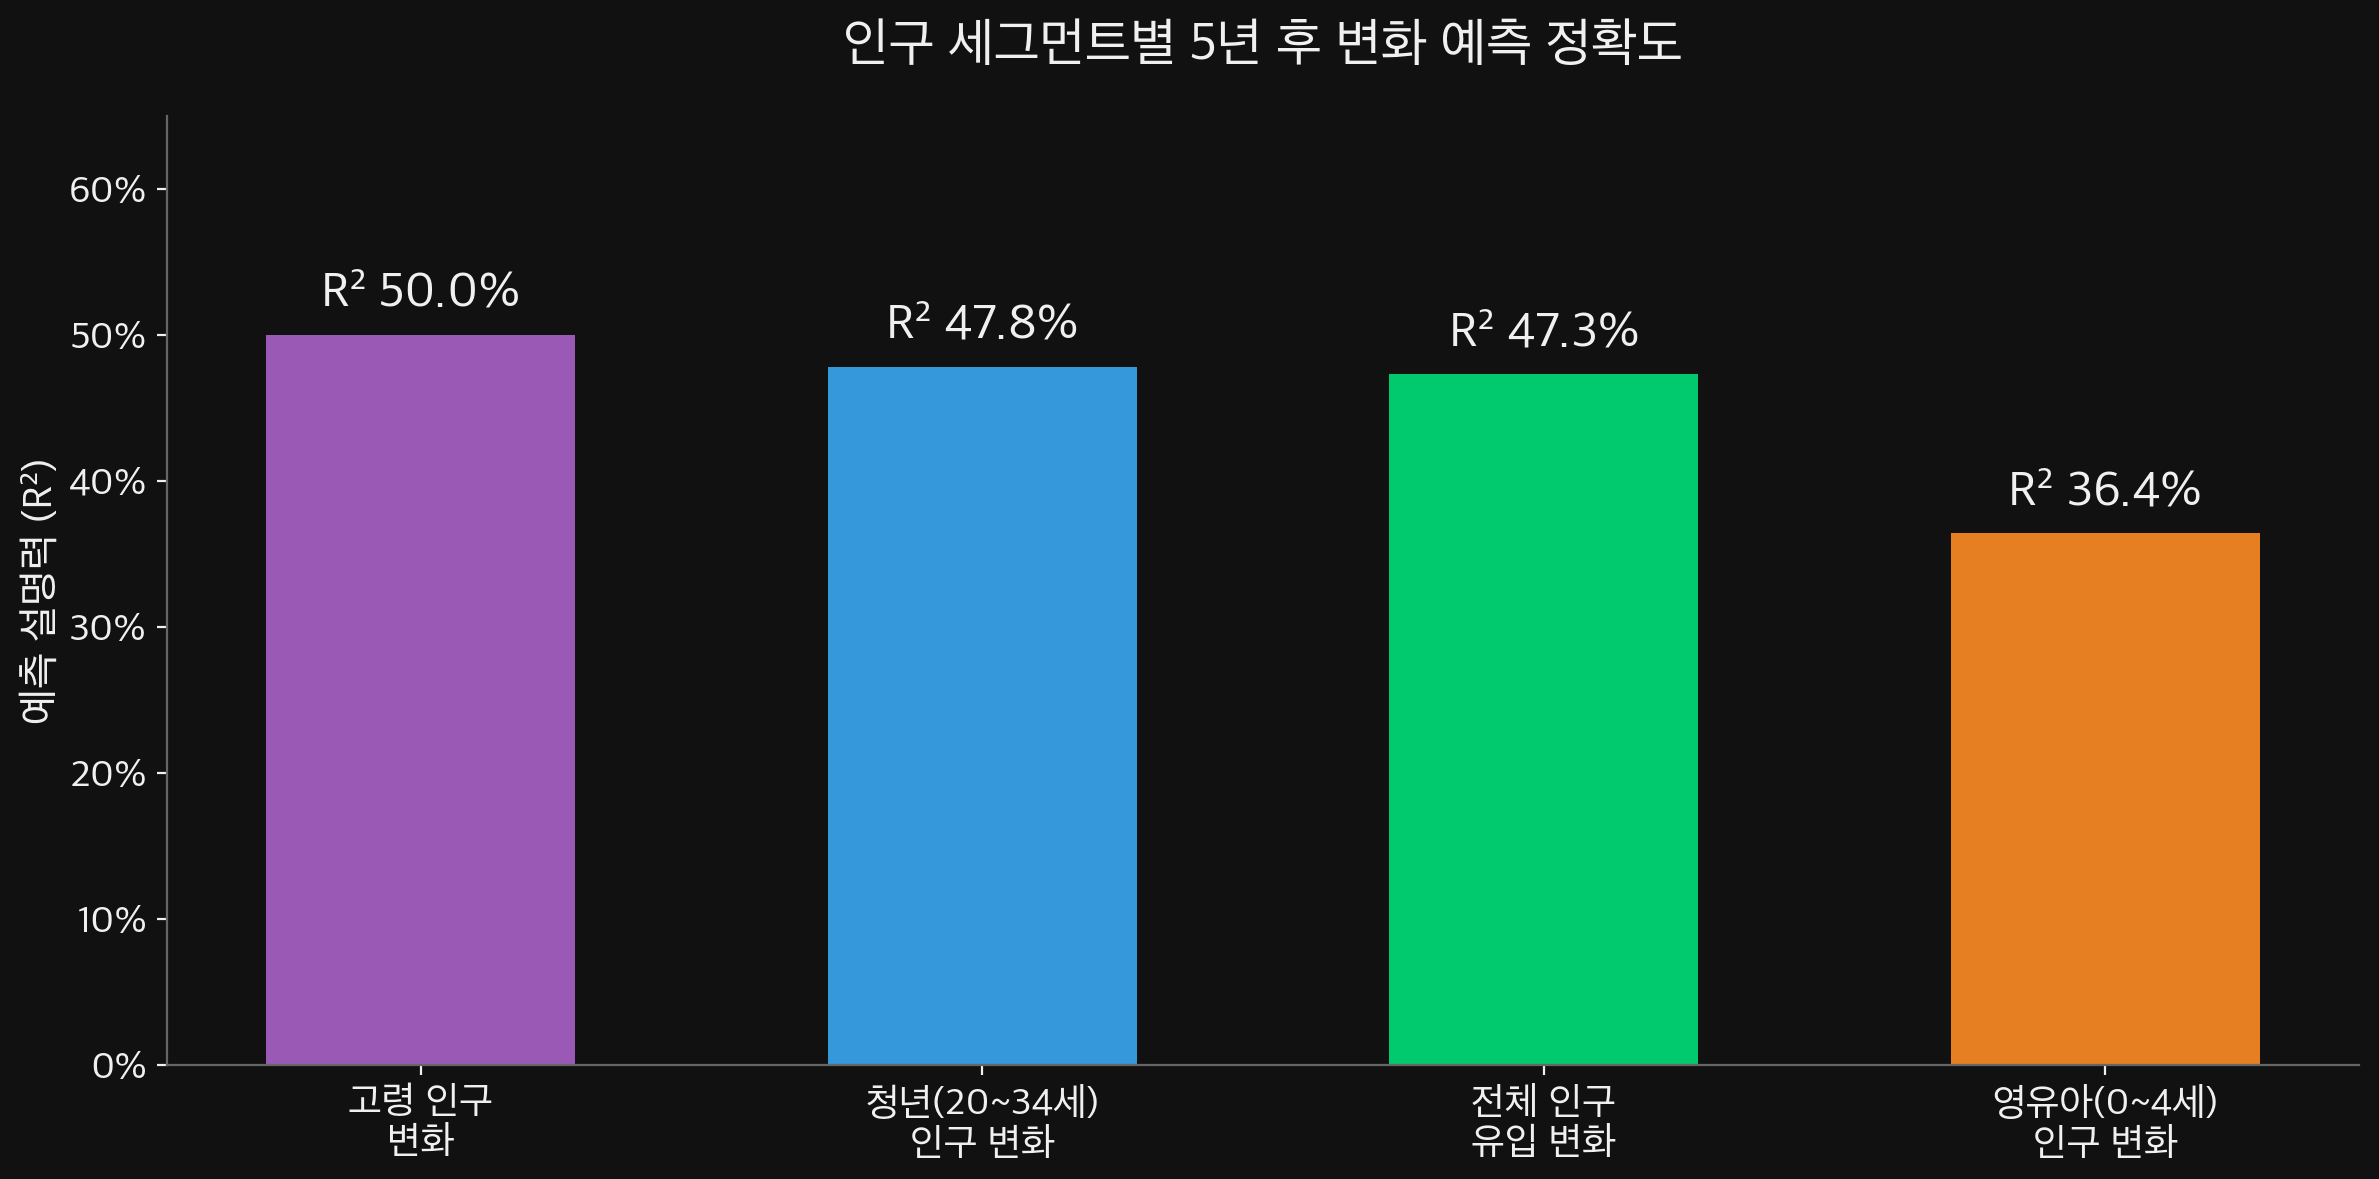
\includegraphics[width=0.92\textwidth]{chart_segment_accuracy.png}
  \caption{인구 세그먼트별 예측 정확도}
\end{figure}

\vspace{0.5em}

\insightbox{고령 인구와 청년 인구의 변동 패턴이 근본적으로 다르다. 고령 인구는 상대적으로 안정적이지만, 청년 인구는 일자리와 교육 인프라에 민감하게 반응하여 변동성이 크다.}

\newpage

% =====================================================================
% PAGE 4: 인구 변동 핵심 요인
% =====================================================================
\section*{인구 변동의 핵심 요인: 악순환 구조}

\vspace{0.5em}

인구 감소는 단일 원인이 아닌, 여러 요인이 서로를 강화하는 \textbf{악순환 구조}에서 발생한다. 그 중심에는 \textbf{일자리}가 있다.

\vspace{1em}

\begin{figure}[H]
  \centering
  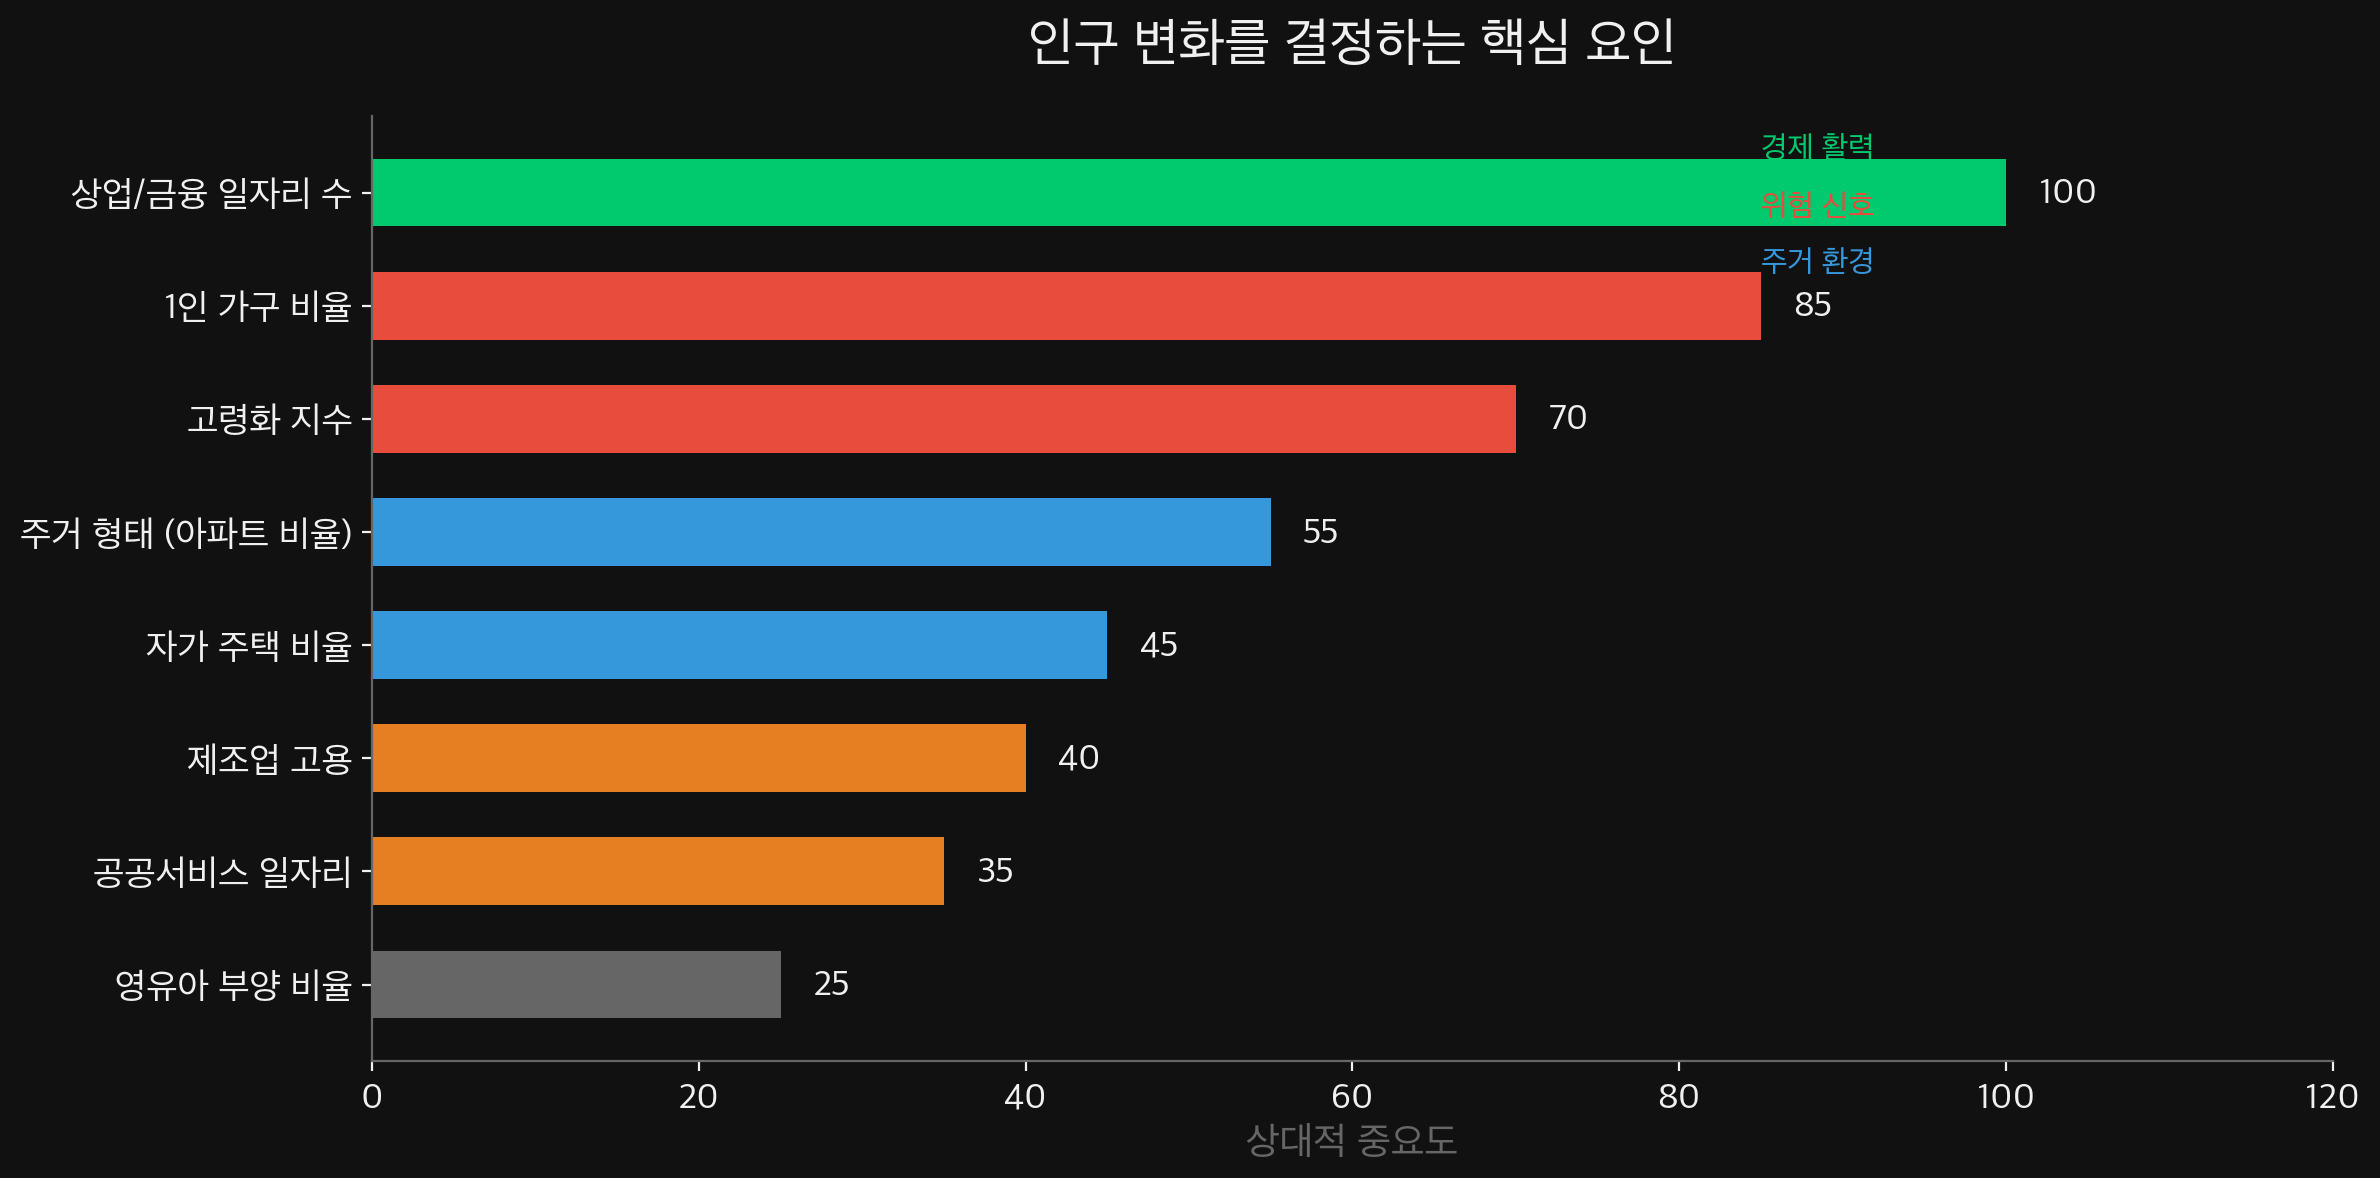
\includegraphics[width=0.92\textwidth]{chart_pop_factors.png}
  \caption{인구 변동의 핵심 예측 요인}
\end{figure}

\vspace{1em}

\noindent
\fcolorbox{bordergray}{lightgray}{%
  \parbox{\dimexpr\textwidth-2\fboxsep-2\fboxrule}{%
    \vspace{0.8em}
    {\large\bfseries\textcolor{darkblue}{악순환의 메커니즘}}\\[8pt]
    \begin{enumerate}[leftmargin=1.5em, itemsep=4pt]
      \item \textbf{일자리 감소} --- 지역 경제 기반 약화
      \item \textbf{청년 유출} --- 취업을 위해 대도시로 이동
      \item \textbf{출산율 하락} --- 가임 인구 감소로 자연 감소 가속
      \item \textbf{고령화 심화} --- 남은 인구의 고령화
      \item \textbf{지역 서비스 축소} --- 인구 감소로 인한 인프라 위축
      \item \textbf{추가 유출} --- 생활 여건 악화로 인한 추가 이탈
    \end{enumerate}
    \vspace{0.6em}
  }%
}

\newpage

% =====================================================================
% PAGE 5: 정책 시사점 + 문의
% =====================================================================
\section*{정책 시사점}

\vspace{0.5em}

\noindent
\fcolorbox{bordergray}{lightgray}{%
  \parbox{\dimexpr\textwidth-2\fboxsep-2\fboxrule}{%
    \vspace{0.8em}
    {\large\bfseries\textcolor{darkblue}{1. 일자리 중심의 지역 활성화 정책}}\\[6pt]
    {\normalsize 인구 감소의 근본 원인은 일자리이다. 출산 장려금 등 단편적 정책보다, 지역에 양질의 일자리를 창출하는 산업 정책이 인구 유지의 핵심이다.}
    \vspace{0.6em}
  }%
}

\vspace{0.8em}

\noindent
\fcolorbox{bordergray}{lightgray}{%
  \parbox{\dimexpr\textwidth-2\fboxsep-2\fboxrule}{%
    \vspace{0.8em}
    {\large\bfseries\textcolor{darkblue}{2. 행정동 단위 맞춤형 정책 설계}}\\[6pt]
    {\normalsize 3,518개 행정동의 인구 변동 패턴은 모두 다르다. 전국 단일 정책이 아닌, 각 지역의 인구 구조와 변동 동인에 맞는 맞춤형 정책이 필요하다.}
    \vspace{0.6em}
  }%
}

\vspace{0.8em}

\noindent
\fcolorbox{bordergray}{lightgray}{%
  \parbox{\dimexpr\textwidth-2\fboxsep-2\fboxrule}{%
    \vspace{0.8em}
    {\large\bfseries\textcolor{darkblue}{3. 예측 기반 선제적 대응}}\\[6pt]
    {\normalsize 인구 변화는 느리지만 되돌리기 어렵다. 5년 후 인구 구조를 미리 예측하여, 인구 감소가 본격화되기 전에 선제적으로 대응하는 것이 비용 효율적이다.}
    \vspace{0.6em}
  }%
}

\vspace{3em}

\begin{center}
\fcolorbox{darkaccent}{lightblue}{%
  \parbox{0.85\textwidth}{%
    \vspace{1em}
    \begin{center}
    {\Large\bfseries\textcolor{darkblue}{전체 보고서 및 상세 분석은}}\\[8pt]
    {\Large\bfseries\textcolor{darkblue}{연구실로 문의해주세요}}\\[12pt]
    {\normalsize\textcolor{gray}{한양대학교 경영대학 임보람 교수 연구실}}\\[4pt]
    {\normalsize\textcolor{gray}{빅데이터 마케팅 연구그룹}}
    \end{center}
    \vspace{1em}
  }%
}
\end{center}

\end{document}
